\documentclass[10pt]{report}
\usepackage[utf8]{inputenc}
\usepackage[spanish]{babel}
\usepackage[top=1.2cm,bottom=1.5cm,left=1.2cm, right=1.2cm,bindingoffset=0.6cm]{geometry}

% Fuente Times New Roman
\usepackage{newtxtext,newtxmath}
% Tamaño de fuente específica
\usepackage{anyfontsize}
% Imágenes
\usepackage{graphicx}
% Justificar texto
\usepackage{ragged2e}
% BibLaTex
\usepackage{biblatex,csquotes}
\addbibresource{Referencias.bib}
% Multiple columns
\usepackage{multicol,blindtext}
% Array package for tables
\usepackage{array}
% Color for tables
\usepackage[table]{xcolor}
\usepackage{colortbl}

\begin{document}

\begin{center}
    \vspace*{1cm}
    
    {\fontsize{14}{16} \textbf{Prototipo embebido de la interpretación de patrones de movimiento en una mano para la reproducción de fonemas y palabras completas en el idioma Español de México}}
    
    \vspace{0.2cm}
    
    {\fontsize{12}{14} \textbf{\textit{Trabajo Terminal No. \_\_\_\_-\_\_\_}} }
    
    \vspace{0.1cm}
    
    \textit{Alumnos: *Valle Martínez Luis Eduardo}
    
    \vspace{0.1cm}
    
    \textit{Directores: Rodolfo Romero Herrera, Dr. Jesús Yaljá Montiél Pérez}
    
    \vspace{0.1cm}
    
    \textit{*e-mail: lvallem1400@alumno.ipn.mx}
    
\end{center}

\hfill\break
\justifying
\textbf{Resumen} - Creación de un sistema embebido basado en RaspberryPi que utiliza el SoC Micro Bit de la BBC como dispositivo sensor, y la tarjeta de sonido adaptada para sistemas RaspberryPi, WM8960 de Waveshare, para la reproducción de los fonemas. La tarjeta Micro Bit se coloca sobre el dorso de la mano permitiendo identificar los movimientos realizados con esta al aprovecharse el sensor de acelerómetro integrado, mientras la transmisión de su recopilación se logra mediante conexión Bluetooth. Los datos adquiridos son procesados con un algoritmo de clasificación basado en \textit{Deep Learning} y DTW(\textit{Dynamic Time Warping}), que permitirpa calcular la coincidencia óptima entre la secuencia recopilada y las secuencias modelos correspondientes a cada fonema para su correcta identificación y finalmente reproducción sonora.

\hfill \break
\textbf{Palabras clave} - Algoritmo DTW(\textit{Dynamic Time Warping}), \textit{Deep Learning}, Reproducción de voz, Sistemas Embebidos

\hfill \break
{\fontsize{12}{14}\textbf{1. Introducción}}
\hfill \break
\input{Secciones/Introducción}

\hfill \break
{\fontsize{12}{14}\textbf{2. Objetivo}}
\hfill \break
\justifying
\hfill\break 
Objetivo general: \hfill\break
Crear un sistema embebido como apoyo a la comunicación a personas con afecciones del habla conformado por un prototipo de \textit{wearable} sensor del movimiento en una mano, un modelo de \textit{Machine Learning} para la clasificación de los patrones y un servicio de \textit{Text-to-Speech} para la reproducción sonora de palabras y frases.

\hfill\break
Objetivos específicos:	
\begin{enumerate}

	\item \justifying Idear un conjunto de patrones de movimientos como código motriz que permita al usuario describir letras del alfabeto para la conformación de palabras y frases.
	
	\item \justifying Ensamblar el prototipo de guante \textit{wearable} sensor implementando el SoC micro:bit para el cambio de aceleraciones y un sensor de pulso para indicar el inicio y fin del muestreo de un movimiento.

	\item \justifying Identificar un modelo de \textit{Machine Learning} que en conjunto al algoritmo DTW clasifiquen eficientemente los patrones de movimiento a clases alfabéticas.
	
	\item \justifying Configurar el servicio local y en la nube de \textit{Text-to-Speech} para la reproducción sonora de las palabras y frases.
\end{enumerate}

\hfill \break
{\fontsize{12}{14}\textbf{3. Justificación}}

\hfill \break
{\fontsize{12}{14}\textbf{4. Productos o Resultados esperados}}

\hfill \break
{\fontsize{12}{14}\textbf{5. Metodología}}

\hfill \break
{\fontsize{12}{14}\textbf{6. Cronograma}}

\hfill \break

\newpage

{\fontsize{12}{14}\textbf{7. Referencias}}

\printbibliography

\hfill \break

\newpage

{\fontsize{12}{14}\textbf{8. Alumnos y Directores}}

\begin{multicols*}{2}
	\hfill \break
	\hfill \break
	\justifying
	\textit{Luis Eduardo Valle Martínez}.- Alumno de la carrera de Ing. en Sistemas Computacionales en ESCOM, Especialidad Sistemas, Boleta: 2015090780, Tel. 5566143276, email: lvallem1400@alumno.ipn.mx
	
	\hfill \break
	\hfill \break
	\centering
	
\includegraphics[width=5cm]{Imagenes/firma.png}
	
	
	Firma: \hrulefill
	
	\hfill \break
	\hfill \break
	\justifying
	\textit{Rodolfo Romero Herrera}.- Profesor de tiempo completo Laboratorio de posgrado Sistemas computacionales móviles. Candidato a Doctor en ciencias en Comunicaciones y Electrónica. Maestría en ciencias en Ingeniería electrónica. Ingeniería en comunicaciones y Electrónica. Área de trabajo Inteligencia Artificial y Procesamiento digital de señales. Tel. 5535216128, email: rromeroh@ipn.mx.
	
	\hfill \break
	\centering
	
\includegraphics[width=5cm]{Imagenes/firma_Rodolfo_Romero.png}
	
	Firma: \hrulefill
	
	\hfill \break
	\hfill \break
	\justifying
	\textit{Jesús Yaljá Montiel Pérez}.- Profesor de tiempo completo adscrito al Laboratorio de Robótica y Mecatrónica del Centro de Investigación en Computación del Instituto Politécnico nacional. Doctor en comunicaciones y electrónica. Maestro en Ciencias en Ingeniería electrónica e Ingeniero Físico. Sus intereses son: la Inteligencia Artificial, sensores y robótica. Tel: 5524940919, Ext. IPN: 56665, email: yalja@ipn.mx
	
	\hfill \break
	\hfill \break
	\centering
	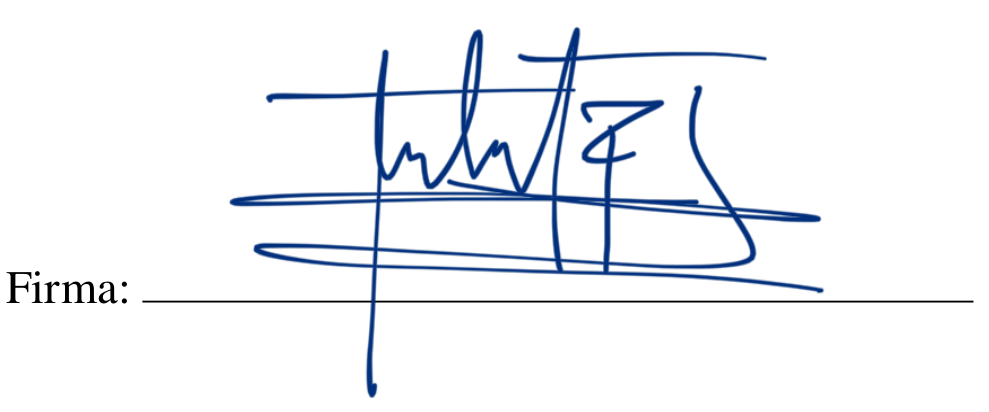
\includegraphics[width=7.9cm]{Imagenes/firma_Jesus_Yalja.png}

	
	
	\begin{tabular}{>{\raggedleft\arraybackslash\columncolor[HTML]{EFEFEF}}p{6.8cm}}
		{\scriptsize CARÁCTER: Confidencial}\\
		{\scriptsize FUNDAMENTO LEGAL: Artículo 11 Fracc. V y Artículos 108, 113 y 117 de la Ley Federal de Transparencia y Acceso} \\
		{\scriptsize a la Información Pública.}\\
		{\scriptsize PARTES CONFIDENCIALES: Número de boleta y teléfono}
	\end{tabular}

\end{multicols*}

\end{document}
